%==================================
% (c) Jan Tulak, 2017
%%%%%%%%%%%%%%%%%%%%%%%%%%%%%%%%%%%%%%%%%%%%%%%%%%%%%%%%%%%%%%%%%%%%%%%%%%%%%

\chapter{Used Techniques and procedures}\label{chap:techniques}
%----------------------------------------------------------------------

In this chapter, we discuss which techniques and models of formal analysis and verification are useful for the code of {\tt mkfs.xfs}. Let us at first define important constraints that are limiting or directing our choice.

We are analysing a single-threaded application. This greatly reduces the
state space and means that we also can use methods that do not allow for
concurrency. On the other side, given that the program accepts user input,
some variables have an infinite number of potential values and any method
based on state space checks must cope with this fact.

%With respect to possible difficulties with implementing various advanced
%methods and their required proficiency, it was decided to start with well-known
%and used tools and gradually move from these production-ready, easy to use
%solutions to tools requiring more of user input.

%Some tools will be used multiple times because while, for example, {\em
%	Coverity} can be used on the whole source of {\em xfsprogs}, other
%	tools like {\em CPAChecker} require modelling of the environment and so
%	for practical reasons, they are run only on an extracted part of {\tt
%		mkfs\_xfs.c}, where things like access to disk devices are
%		removed to create a maximally self-contained code. This means
%		that we are not able to detect errors in some parts of the
%		code, but it is nearly impossible to model and test a whole
%		operating system and we have to make the cut somewhere.
%
%Thus, to be able to compare the various tools directly, some of the tools are run both on the full code as well as on the dissected part.

A comparison that could be interesting for further research is to experiment
with tools that use neural networks and deep learning as an integral part of
their algorithms if such tools exist. Examples of the use of those technologies
are a heuristic to drive the selection of inference rules in theorem proving,
or spotting error patterns~\footnote{Some attempts in modelling a code are
hinted in {\em On the Naturalness of Software} by Abram Hindle:
\url{http://dl.acm.org/citation.cfm?id=2902362}.} However, these approaches are
even more complex and experimental than the traditional approaches and
would probably deserve a standalone work on their own.
% TODO http://dl.acm.org/citation.cfm?id=2902362 download and read... search for deep learning sources

List of tools that were used in this work (in no particular order): Coverity,
CppCheck and the analysis in GCC and Clang compilers.


%======================================================================
\section{Testing Environment}\label{chap:techniques:env}
%----------------------------------------------------------------------

The tools were run in a Docker container\footnote{Simply stated, a
	container is an image that has been started, similar to the
		difference between a running virtual machine and its
		on-disk virtual HDD image. Unlike virtualization,
		containers are only processes isolated from the rest of the
system using kernel capabilities, like {\em cgroups} and {\em chroot}.
Docker is a specific implementation~\cite{docker} of containers.} based on Fedora Linux
25. The use of containers ensures a clean and identical environment for
every tool and every run. Image with the compilers and CppCheck are published
in Docker Hub and all the recipes to build and use them are provided with
this work. Image with Coverity could not be published because it contains
confidential information\footnote{Jan Ťulák had an access to Red Hat Coverity license
server as a Red Hat employee. However, the server information and some tools
	Red Hat provided with Coverity are considered confidential.}.

Every image has its own starting script for easier manipulation -- {\tt
run.sh}.  This script creates a container from the image and mounts the
directory with xfsprogs (or any other directory which is passed to it).
Then, if necessary, it can pass few options to the script started in
the container.

{\tt run-test.sh} is the script started by Docker after creating the container.
This script copies xfsprogs from the mounted directory to another one, so it
does not change the original repository in any way. In this copied directory
the script then starts whatever tool it is prepared for.

Users can, if they wish to do so, enter an interactive shell in the container
instead of starting the tool. Also, it is possible to skip the copying or to
run {\tt make clean}. For an automated run described in
\Cref{chap:techniques:processing}, neither of this is necessary, but these
options are useful for manual experiments.


Coverity, GCC and Clang are run using {\tt csbuild}, a tool to plug static
analyzers into the build process~\cite{csbuildMan}. Because csbuild attempts to
use all supported analyzers it finds, the images for each tool we are testing
are modified to contain only the single specific tool we need, but no other.
%%_____________________________________________________
%\subsection{CPAChecker}
%%.....................................................
%Docker image: {\tt jtulak/cpacheck}~\cite{dockerCPAChecker}
%
%CPAChecker can not be run on a full source code tree, but requires
%preprocessing~\cite{cpacheckerGettingStarted}, which must be partially
%remade for every tested revision (depending on what and how much changed),
%       only selected commits were tested.
%_____________________________________________________
\subsection{CppCheck}
%.....................................................
Docker image: {\tt jtulak/cppcheck}~\cite{dockerCPPCheck}

CppCheck is also used in {\em Codacy}, an automated code review application
with Github integration. Results from Codacy are included for comparison.

Because CppCheck does not need preprocessed code, it was reasonable to use
it for every commit in our changes.

When running this tool, default configuration was used, and all types of
messages were enabled. No custom rules were used and the invocation of
CppCheck on whole {\tt xfsprogs/mkfs/} directory was:

{\tt cppcheck --enable=all mkfs/}


%_____________________________________________________
\subsection{Coverity}
%.....................................................
Coverity was used both manually in a Docker container, and automatically
using the public Coverity service for open source projects which is part
of the standard xfsprogs development process, to compare the results between
those two instances.

Furthermore, in the local analysis, four levels of analysis aggressiveness were
tested: low (default settings), medium, high and custom (all). The different
results are compared in \Cref{chap:results:coverity}, where were look at a
summary of what these levels enabled. With a higher level, Coverity makes more
aggressive assumptions during the analysis, which means more defects being
reported and longer analysis time~\cite{coverityMan}.

Coverity manual claims false positive rate for all checkers that are not parse
warnings increases approximately by 50\% for medium and by 70\% for high. It
does not have an effect on parse warnings checkers.

All levels have enabled everything that a previous, lower level has, plus some
additional checks. The medium level uses low level plus enables some other
checks, including parse warnings, infinite loops, some resource leaks checks,
etc. The high level then adds e.g. integer overflow detections and more checks
for infinite loops. A special, level enabled by {\tt --all} flag for {\tt
cov-analysis}, then enables almost all checkers, with only a few minor
exceptions. For the full (rather long) list of what checkers are enabled on every
level, consult the {\tt cov-analysis} manual~\cite{coverityMan}.

\begin{figure}
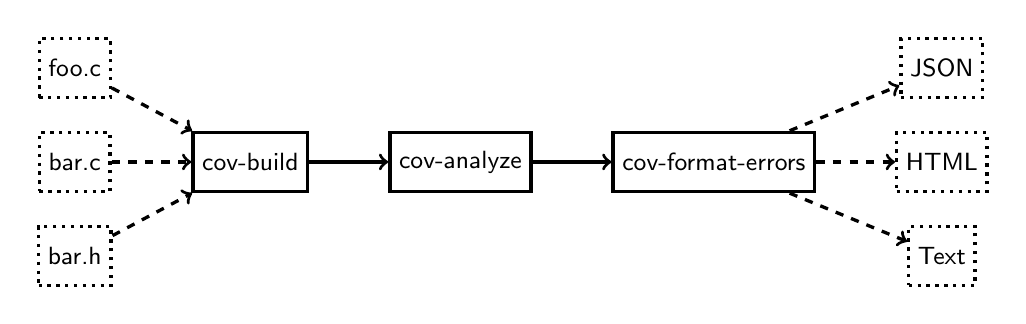
\begin{tikzpicture}

\matrix [column sep=10mm, row sep=4mm, every node/.style={
    shape=rectangle,
    minimum height=0.75cm,
    text centered,
    font=\sffamily\small,
    very thick,
    color=black,
    draw=black,
    fill=white,
}] {
  \node[dotted] (a1) {foo.c}; & & & &
  \node[dotted] (a5) {JSON}; \\

  \node[dotted] (b1) {bar.c}; &
  \node (b2) {cov-build}; &
  \node (b3) {cov-analyze}; &
  \node (b4) {cov-format-errors}; &
  \node[dotted] (b5) {HTML}; \\

  \node[dotted] (c1) {bar.h}; & & & &
  \node[dotted] (c5) {Text}; \\
};

\begin{scope}[->, very thick, black]
  \draw[dashed] (a1) -- (b2);
  \draw[dashed] (b1) -- (b2);
  \draw[dashed] (c1) -- (b2);
  \draw (b2) -- (b3);
  \draw (b3) -- (b4);
  \draw[dashed] (b4) -- (a5);
  \draw[dashed] (b4) -- (b5);
  \draw[dashed] (b4) -- (c5);
\end{scope}

\end{tikzpicture}
\caption{Process steps for coverity analysis.}
\label{fig:techniques:coverity:steps}
\end{figure}

The \Cref{fig:techniques:coverity:steps} describes the steps happening in
Coverity container. Where other tools are only a single step, taking source
code on one side and producing an output on the other side, Coverity has three
standalone steps. First, it builds the source code using its own parser and
produces an analyzable data. 

The second step, {\tt cov-analyze} application, does the analysis itself. Here
it is possible to set up the aggressiveness level and where the license is
required. The last step then takes the raw output from the analyser and
converts it into one of the selected formats. The scripts in the container
generate all three variants. Due to the size of the HTML output, it is not
included in the digital attachment to this work.

%_____________________________________________________
\subsection{GCC}
%.....................................................
The {\em GNU project C and C++ compiler} is used for compiling xfsprogs and it
has some static analysis capabilities because it must understand the code to
compile it. The only difference in its use from standard configuration is to
use the most strict reporting.

%_____________________________________________________
\subsection{Clang}
%.....................................................
Clang is another C/C++ compiler. It was founded by Apple and LLVM communities
in 2007 as an alternative to GCC, which did not work well for Apple's needs. It
is designed to be highly compatible with GCC for C-based languages (C, C++,
ObjC), but does not have the desire to replace it
completely~\cite{ClangAnnouncement}.

It is not used by xfsprogs but can compile the code as well, so we can compare
it with GCC and other analysis tools. Even if it has its analyzing part as a
standalone application~\cite{ClangAnalyser}, the easiest way to use it and to
make it the most comparable with GCC was to rename clang binary to GCC and let
xfsprogs behave as if it was GCC, rather than modify Autotools configuration.
According to Clang's {\tt scan-build} description, the tool replaces certain
environmental variables to achieve the same result. However, from the nature of
tool-specific containers used for the tests, binary replacement avoids
uncertainty about whether the environmental variables were correctly taken into
the account in this specific Autotools configuration without the usual
consequences of manipulating with system files without the knowledge of a
package manager.

%======================================================================
\section{Results Processing}\label{chap:techniques:processing}
%----------------------------------------------------------------------
The outputs of these tools have different syntax and verbosity, but we had to
find a way, how to compare them, both between the tools and across revisions,
     despite some of the tools finding a lot of issues. A set of
     scripts to help both with automating the tests and with analysing was
     created. The \Cref{fig:techniques:steps} shows how these scripts are
     connected with what happens in the containers.

First, there is tool {\tt parse.py}, which can automatically run all the tools
across specified revisions. It takes care of changing the revisions, starting
every docker container again and finally, it organises the outputs in a logical
way: in a specified directory, it creates a subdirectory for every revision
(using the revision's short hash as the directory name) and each such directory
then contains log files with outputs from each tool.

\begin{figure}
\begin{tikzpicture}

\matrix [column sep=8mm, row sep=15mm, every node/.style={
    shape=rectangle,
    minimum height=0.75cm,
    text centered,
    font=\sffamily\small,
    very thick,
    color=black,
    draw=black,
    fill=white,
}] {
  \node[dotted] (a1) {source code}; & &
  \node[dotted] (a3) {output files}; &
  \node (a4) {format-outputs.sh}; &
  \node (a5) {parse.py}; \\

  \node (b1) {copy to container}; &
  \node (b2) {analyze}; &
  \node (b3)[text width=3cm] {move the results out of the container}; \\
};

\begin{scope}[->, very thick, black]
  \draw (a1) -- (b1);
  \draw (b1) -- (b2);
  \draw (b2) -- (b3);
  \draw (b3) -- (a3);
  \draw (a3) -- (a4);
  \draw (a4) -- (a5);
  \node (X)[draw=black,dashed,inner sep=0.50cm, fit= (b1) (b3)] {};
  \node [inner sep=0.30cm, fit= (b1) (b3),yshift=0.6ex,] at (X.south) {tests.py};
\end{scope}

\end{tikzpicture}
\caption{Process steps for testing.}
\label{fig:techniques:steps}
\end{figure}

The output files are not modified in the first step, but to simplify their
parsing, it is useful to preprocess some of those files (namely from GCC and
	/						 Clang) with script
{\tt format-outputs.sh}, to remove color formatting escape sequences and
unnecessary compiler outputs.  Such data may be useful for some further
analysis, but for the next step, it would only make the parsing more complex.

In the last step, script {\tt parse.py}, when supplied with the output
directory, translates the different syntaxes into a single inner
representation, which can be then used to simply compute deltas between
different revisions.

The algorithms to complete these deltas has one known issue: if there are
multiple issues with the same message (e.g. because variable with name {\tt
				       foo} was declared, but not used, in
				       multiple functions) and later some of
these issues are fixed, the number of issues is correct, but the indicated
lines may be incorrect. This is because the script must cope with changing
code; an issue on line X in one revision can be on line Y in another one, and
that would require employing much more complex algorithms that would use
information from git and understand which lines moved where. Thus, in such
cases, the behaviour selecting specific instances of the same kind of issue is
undefined.


%The classification of issues into one of the style, error or security category
%is only indicative. For GCC and Clang, it is based on what specific flag for the
%compiler enables reporting of any specific issue. We attempted to estimate what
%consequences can these issues have in general, whether they can cause a bigger
%problem, or if their greatest danger is in being misleading or not a good
%practice.
%
%From the issues found in whole xfsprogs, we configured only one compiler flag
%to be detected as something else than style issue: {\tt -Wfloat-equal}.
%Directly comparing two floats is not reliable due to their representation
%in memory~\cite{floatsComparing}. Thus, this kind of issue is certainly
%something that can work differently than expected and deserves more
%attention, than, say, shadowing a global variable with a local one.
%
%This kind of issue was not found in mkfs itself and in xfsprogs, it appears
%only in two places, both to set the precision of a printf. In other words,
%the only occurrences of direct comparison of floats are intentional testing
%for imprecise numbers and can be considered false positives in the context
%of the program. Clang finds this issue as well. In comparison, Coverity
%does not raise it and it seems that it can somehow infer the intention of
%the use.
%
%For CppCheck, the classification uses the category reported by CppCheck itself:
%If CppCheck reports an issue as anything else than style issue, it is
%considered a potential error, but it did not report anything else than style
%issue. Coverity reports also a categorization. In xfsprogs, the only two
%categories that were reported are quality and security.

Finally, while it is possible to find differences between revisions within the
results of a single tool, albeit with the small instability in case of multiple
similar entries mentioned above, doing this between tools on a single revision
proved a much more complex task. Every tool describes the same issue with
different words, so to be able to automatically compute any differences, such
an algorithm would have to understand the issue in all details. Thus,
cross-tool differences are not computed automatically, but manually for the
cases where it is reasonable given to the number of issues that must be
analysed. Standard Unix tools like {\tt diff} and {\tt grep} were used in these
cases.
